% Standalone TikZ figure for Reversible Gauge Transformer architecture
% Compile with: pdflatex architecture.tex
\documentclass[tikz,border=10pt]{standalone}
\usepackage{tikz}
\usepackage{amsmath,amssymb}
\usepackage{bm}
\usetikzlibrary{arrows.meta,positioning,shapes.geometric,decorations.pathmorphing,calc,fit,backgrounds,patterns}

\begin{document}
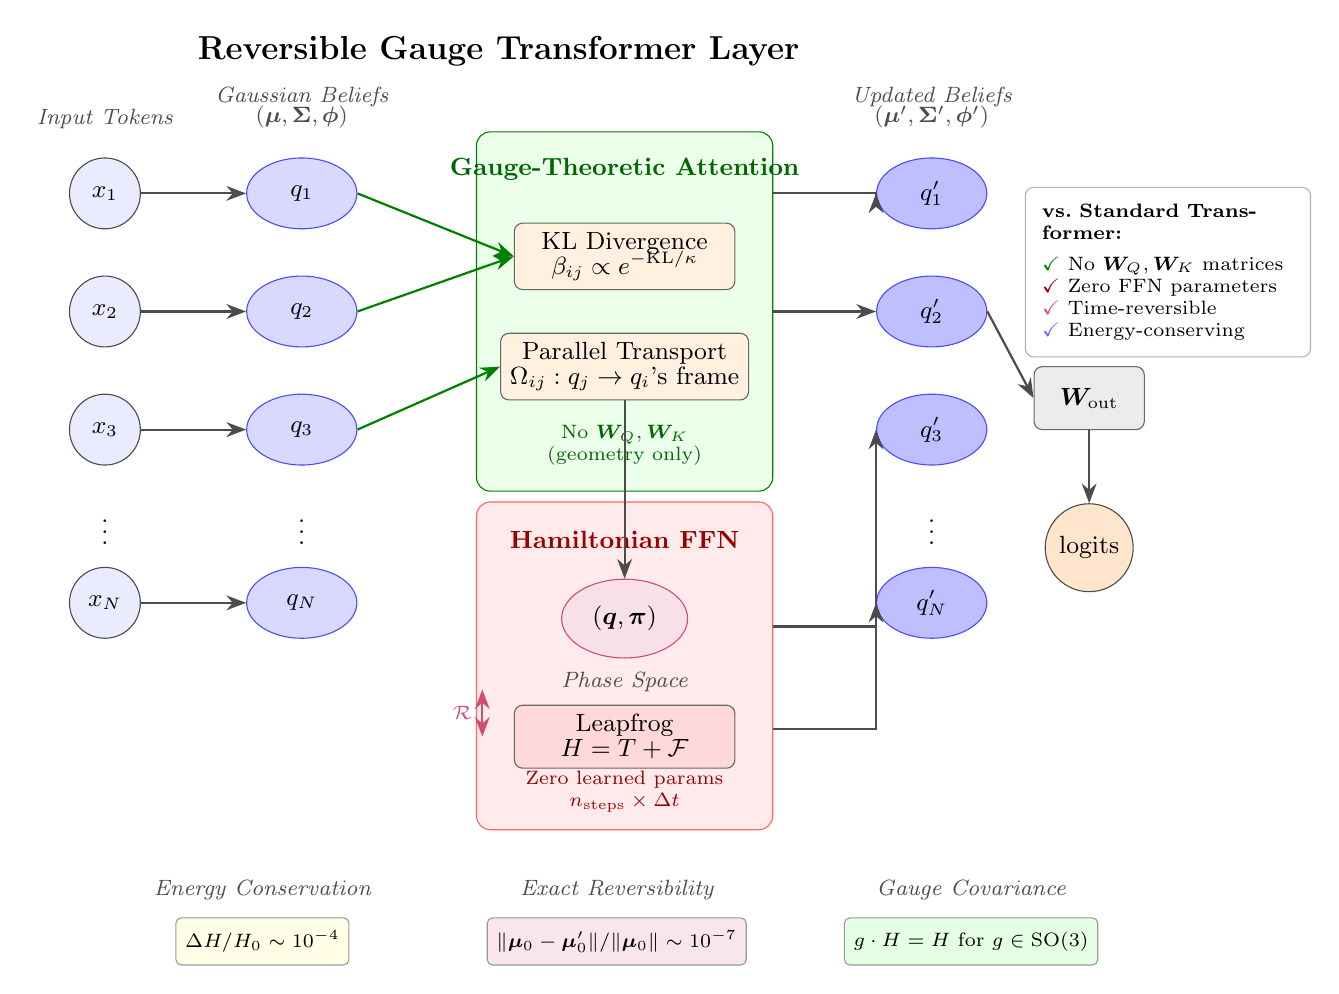
\begin{tikzpicture}[
    % Node styles
    token/.style={circle, draw=black!70, fill=blue!8, minimum size=0.9cm, font=\small},
    belief/.style={ellipse, draw=blue!70, fill=blue!15, minimum width=1.4cm, minimum height=0.9cm, font=\small},
    phase/.style={ellipse, draw=purple!70, fill=purple!12, minimum width=1.6cm, minimum height=1cm, font=\small},
    process/.style={rectangle, rounded corners=3pt, draw=black!60, fill=orange!12, minimum width=2.2cm, minimum height=0.8cm, font=\small, align=center},
    hambox/.style={rectangle, rounded corners=5pt, draw=red!60, fill=red!8, minimum width=3.2cm, minimum height=2.4cm},
    attnbox/.style={rectangle, rounded corners=5pt, draw=green!50!black, fill=green!8, minimum width=3.2cm, minimum height=1.6cm},
    label/.style={font=\footnotesize\itshape, text=black!70},
    arrow/.style={-{Stealth[length=2.5mm]}, thick, black!70},
    dasharrow/.style={-{Stealth[length=2.5mm]}, thick, black!50, dashed},
    reversearrow/.style={{Stealth[length=2.5mm]}-{Stealth[length=2.5mm]}, thick, purple!70},
    curvearrow/.style={-{Stealth[length=2.5mm]}, thick, green!50!black, bend left=20},
]

% ============================================================================
% Title
% ============================================================================
\node[font=\large\bfseries] at (5, 5.8) {Reversible Gauge Transformer Layer};

% ============================================================================
% Input tokens (left side)
% ============================================================================
\node[token] (t1) at (0, 4) {$x_1$};
\node[token] (t2) at (0, 2.5) {$x_2$};
\node[token] (t3) at (0, 1) {$x_3$};
\node[font=\small] at (0, -0.2) {$\vdots$};
\node[token] (tn) at (0, -1.2) {$x_N$};

\node[label, anchor=south] at (0, 4.7) {Input Tokens};

% ============================================================================
% Gaussian beliefs (after embedding)
% ============================================================================
\node[belief] (b1) at (2.5, 4) {$q_1$};
\node[belief] (b2) at (2.5, 2.5) {$q_2$};
\node[belief] (b3) at (2.5, 1) {$q_3$};
\node[font=\small] at (2.5, -0.2) {$\vdots$};
\node[belief] (bn) at (2.5, -1.2) {$q_N$};

\node[label, anchor=south, align=center] at (2.5, 4.7) {Gaussian Beliefs\\[-2pt]$(\bm{\mu}, \bm{\Sigma}, \bm{\phi})$};

% Arrows: tokens to beliefs
\draw[arrow] (t1) -- (b1);
\draw[arrow] (t2) -- (b2);
\draw[arrow] (t3) -- (b3);
\draw[arrow] (tn) -- (bn);

% ============================================================================
% KL-Attention box
% ============================================================================
\begin{scope}[on background layer]
    \node[attnbox, fit={(5, 4.5) (8.2, 0.5)}, inner sep=8pt] (attnbg) {};
\end{scope}
\node[font=\small\bfseries, green!40!black] at (6.6, 4.3) {Gauge-Theoretic Attention};

% Attention internals
\node[process, minimum width=2.8cm] (kl) at (6.6, 3.2) {KL Divergence\\[-2pt]$\beta_{ij} \propto e^{-\mathrm{KL}/\kappa}$};

\node[process, minimum width=2.8cm] (transport) at (6.6, 1.8) {Parallel Transport\\[-2pt]$\Omega_{ij}: q_j \to q_i$'s frame};

% Label: no W_Q, W_K
\node[font=\scriptsize, text=green!40!black, align=center] at (6.6, 0.8) {No $\bm{W}_Q, \bm{W}_K$\\(geometry only)};

% Curved arrows showing attention between beliefs
\draw[curvearrow] (b1.east) to[out=0, in=180] (kl.west);
\draw[curvearrow] (b2.east) to[out=0, in=180] (kl.west);
\draw[curvearrow] (b3.east) to[out=0, in=180] (transport.west);

% ============================================================================
% Hamiltonian FFN box
% ============================================================================
\begin{scope}[on background layer]
    \node[hambox, fit={(5, -0.2) (8.2, -3.8)}, inner sep=8pt] (hambg) {};
\end{scope}
\node[font=\small\bfseries, red!60!black] at (6.6, -0.4) {Hamiltonian FFN};

% Phase space representation
\node[phase] (phase) at (6.6, -1.4) {$(\bm{q}, \bm{\pi})$};
\node[label, anchor=north] at (6.6, -1.95) {Phase Space};

% Leapfrog integrator
\node[process, fill=red!15, minimum width=2.8cm] (leapfrog) at (6.6, -2.9) {Leapfrog\\[-2pt]$H = T + \mathcal{F}$};

% Label: zero parameters
\node[font=\scriptsize, text=red!60!black, align=center] at (6.6, -3.6) {Zero learned params\\$n_{\mathrm{steps}} \times \Delta t$};

% Arrow from attention to Hamiltonian
\draw[arrow] (transport.south) -- ++(0, -0.5) -| (phase.north);

% Reversibility arrows
\draw[reversearrow] ($(leapfrog.west) + (-0.4, 0)$) -- ($(leapfrog.west) + (-0.4, 0.6)$)
    node[midway, left, font=\scriptsize, text=purple!70] {$\mathcal{R}$};

% ============================================================================
% Output beliefs
% ============================================================================
\node[belief, fill=blue!25] (o1) at (10.5, 4) {$q'_1$};
\node[belief, fill=blue!25] (o2) at (10.5, 2.5) {$q'_2$};
\node[belief, fill=blue!25] (o3) at (10.5, 1) {$q'_3$};
\node[font=\small] at (10.5, -0.2) {$\vdots$};
\node[belief, fill=blue!25] (on) at (10.5, -1.2) {$q'_N$};

\node[label, anchor=south, align=center] at (10.5, 4.7) {Updated Beliefs\\[-2pt]$(\bm{\mu}', \bm{\Sigma}', \bm{\phi}')$};

% Arrows from boxes to output
\draw[arrow] (attnbg.east) ++(0, 1.5) -| (o1.west);
\draw[arrow] (attnbg.east) ++(0, 0) -- (o2.west);
\draw[arrow] (hambg.east) ++(0, 0.5) -| (o3.west);
\draw[arrow] (hambg.east) ++(0, -0.8) -| (on.west);

% ============================================================================
% Output projection
% ============================================================================
\node[process, fill=gray!15, minimum width=1.4cm] (proj) at (12.5, 1.4) {$\bm{W}_{\mathrm{out}}$};
\node[token, fill=orange!20] (logits) at (12.5, -0.5) {logits};

\draw[arrow] (o2.east) -- (proj.west);
\draw[arrow] (proj.south) -- (logits.north);

% ============================================================================
% Key properties (bottom legend)
% ============================================================================
\begin{scope}[shift={(0, -5.5)}]
    % Energy conservation
    \node[draw=black!40, rounded corners=2pt, fill=yellow!10, minimum height=0.6cm, font=\scriptsize] (e1) at (2, 0)
        {$\Delta H / H_0 \sim 10^{-4}$};
    \node[label, anchor=south] at (2, 0.4) {Energy Conservation};

    % Reversibility
    \node[draw=black!40, rounded corners=2pt, fill=purple!10, minimum height=0.6cm, font=\scriptsize] (e2) at (6.5, 0)
        {$\|\bm{\mu}_0 - \bm{\mu}'_0\| / \|\bm{\mu}_0\| \sim 10^{-7}$};
    \node[label, anchor=south] at (6.5, 0.4) {Exact Reversibility};

    % Gauge covariance
    \node[draw=black!40, rounded corners=2pt, fill=green!10, minimum height=0.6cm, font=\scriptsize] (e3) at (11, 0)
        {$g \cdot H = H$ for $g \in \mathrm{SO}(3)$};
    \node[label, anchor=south] at (11, 0.4) {Gauge Covariance};
\end{scope}

% ============================================================================
% Comparison callout
% ============================================================================
\begin{scope}[shift={(13.5, 3)}]
    \node[draw=black!30, rounded corners=3pt, fill=white, align=left, font=\scriptsize,
          inner sep=6pt, text width=3.2cm] (compare) at (0, 0) {
        \textbf{vs.\ Standard Transformer:}\\[3pt]
        \textcolor{green!50!black}{\checkmark} No $\bm{W}_Q, \bm{W}_K$ matrices\\
        \textcolor{red!60!black}{\checkmark} Zero FFN parameters\\
        \textcolor{purple!70}{\checkmark} Time-reversible\\
        \textcolor{blue!60}{\checkmark} Energy-conserving
    };
\end{scope}

\end{tikzpicture}
\end{document}
